\documentclass{article}
\usepackage[preprint]{nips_2018}

\usepackage{graphicx}
\usepackage{hyperref}
\usepackage{amsmath,amssymb}
\usepackage{array}
\usepackage{subcaption}

\usepackage{natbib}
\bibliographystyle{unsrtnat}

\title{Exploring molecular embeddings for cancer drug screening}
\date{\today}
\author{Neil Thomas}

\begin{document}
\maketitle

\section{Introduction}

There is great demand for new compounds that could be used as drugs to treat disease. Drugs may be precisely targeted to subpopulations, or that can circumvent disease resistance. In addition, drugs may have many negative side effects: can similar therapeutic effects be found in different compounds with fewer side effects?

Testing massive libraries with hundreds of thousands of compounds for their biological effects is time consuming and expensive. To reduce this cost, recent research computationally explores the space of compounds using generative models (e.g. variational autoencoders). The parameter space of these generative models can be optimized over to maximize or specify the output of a predictor function (e.g. drug effect) as in \citet{Brookes2018, Gomez-Bombarelli2018}. Chemistry suffers from a problem similar to biology, natural language, and natural images: there are massive unlabeled datasets, and very few corresponding labeled datasets. For this reason, unsupervised and semi-supervised modeling approaches hold promise for helping models predict function from chemical structure.

Another promising avenue for meaningfully summarizing structural similarity follows research from natural language processing, and the learning of word and document embeddings as in \citet{Goldberg2014}. By drawing the analogy of graphical substructures (rooted subgraphs) within a complete graph as ``words'' within a ``document'', similar intuition can be applied to learning $\delta$-dimensional continuous embeddings for arbitrary graph structures, deemed \textit{graph2vec} by \citet{Narayanan}. Graphs with similar substructures are similar graphs, and are close (in a Euclidean distance sense) in the embedding space. Since molecules can be represented as graphs, \textit{graph2vec} embeddings can take advantage of large, unlabeled molecular datasets to learn rich embeddings that capture structural similarity between molecules. This also circumvents one of the problems with learning molecular embeddings via complicated strings written in Simplified Molecular-Input Line-Entry System (SMILES) as in \citet{Gomez-Bombarelli2018}. \textit{graph2vec} does not need to learn the complex chemical syntax of SMILES. ``Word'' embeddings for n-grams of amino acids and nucleotides have already shown promise for being able to meaningfully ,capture biophysical characteristics of proteins and DNA sequences such as in \citet{Hamid2018, Asgari2015}.

In this paper we examine the use of \textit{graph2vec} as a means for refining compound screens.

\section{Methods}

\subsection{Word Embeddings or \textit{word2vec}}

Finding vector-space embeddings for words from large text corpora is an essential pre-processing step for any downstream Natural Language Processing (NLP) task (text prediction, sentiment analysis, etc). The fundamental algorithm for determining word embeddings developed in \citet{Mikolov} is known as \textit{word2vec}. The objective of the \textit{word2vec} model (parameterized by $\theta$) is: given a word $w_t$, to maximize the log-likelihood of the context $c = [w_{t-c}, ... , w_{t+c}]$, i.e.

\begin{equation*}
\arg\max_\theta \sum_{t=1}^T \log Pr(w_{t-c}, ... , w_{t+c} | w_t ; \theta)
\end{equation*}

The underlying assumption of this model is the \textit{Distributional Hypothesis}, which states that \textit{words that occur in the same contexts tend to have similar meanings}. Assuming the context words are independent of one another (the ``bag of words'' model) given the target word, the log probability can be rewritten

\begin{equation*}
\arg\max_\theta \sum_{t=1}^T \sum_{\substack{c \le j \le c \\ j \ne 0}} \log Pr(w_{t+j} | w_t ; \theta)
\end{equation*}

For learning word embeddings, $Pr(w_{t+j} | w_t)$ can be written as a softmax over the dot-product of $\delta$-dimensional word embeddings, i.e. their vector representations $v_w \in \mathcal{R^\delta}$

\begin{equation*}
Pr(w_{t+j} | w_t) = \dfrac{\exp(v_{w_t} \cdot v_{w_{t+j}})}{\sum_{w\in\mathcal{V}} \exp(v_{w_t} \cdot v_{w})}
\end{equation*}

Where $\mathcal{V}$ is the vocabulary size.

Training this model can be inefficient, as it involves computing a sum over a very large vocabulary $\mathcal{V}$ at every step. Instead, word embedding models are trained using a procedure known as negative sampling.

\subsection{Negative Sampling}

The goal of negative sampling is to maximize the probability that observed (word, context) pairs are classified as coming from the data $Pr(D=1 | w, c ; \theta)$, and similarly to minimize the probability the (word, context) pairs sampled from a negative distribution $\mathcal{D^\prime}$ are classified as coming from the data.

\begin{equation*}
\arg\max_\theta \sum_{(w, c) \in \mathcal{D}} \log Pr(D = 1 | c, w ; \theta)
+ \sum_{(w, c) \in \mathcal{D^\prime}} \log Pr(D = 0 | c, w ; \theta)
\end{equation*}

In practice these are usually sampled at random from the vocabulary. The probabilities can be rewritten in terms of the vector embeddings

\begin{equation*}
\arg\max_\theta
\sum_{(w, c) \in \mathcal{D}}
    \log \dfrac{1}{1 + \exp{(-v_c \cdot v_w)}}
+ \sum_{(w, c) \in \mathcal{D^\prime}}
    \log \dfrac{1}{1 + \exp{(v_c \cdot v_w)}}
\end{equation*}

In practice more than one negative sample corresponds to each positive sample. This objective encourages similar words to be mapped to similar vectors, while dissimilar words (i.e. words appearing in dissimilar contexts) to be mapped to dissimilar vectors.

Note that the parameters of the model $\theta$ are precisely the word embeddings $v_w$. The output classification probability can be represented as a neural network that takes as input two one-hot encoded words $w$ and $w^\prime$ sampled from the context, maps to the vector representation of those words via a ``representation'' matrix $w^\top R = v_w$ and ${w^\prime}^\top R = v_{w^\prime}$, and then takes the inverse-logit of their dot product to get the classification probabilities. A negative cross-entropy loss function can then be used to back-propagate gradients through the network to train.

\subsection{Document Embeddings or \textit{doc2vec}}

An extension to \textit{word2vec} for learning embeddings of arbitrary length word sequences (sentences, paragraphs, documents) was proposed by \citet{Le2014}. In their distributed bag of words model, for a document $d_i$ with length $l_i$ composed of words $\{w_1, ..., w_{l_i}\}$ the model maximizes

\begin{equation*}
\arg\max_\theta \sum_{j=1}^{l_i} \log Pr(w_j | d_i ; \theta)
\end{equation*}

Where again the probability is defined by a softmax as before. Both the documents $d$ and words $w$ are embedded in a $\delta$-dimensional space, i.e. $v_d, v_w \in \mathcal{R}^\delta$. At each iteration of training, a text window is sampled from the document $D$, and a random word is sampled from that window. A classification task is then formed using that word.


\subsection{Graph Embeddings or \textit{graph2vec}}

The problem statement here follows precisely the statement in the \textit{graph2vec} paper by \citet{Narayanan} (Section 2). We give the intuition here. For a given graph $G = (N, E, \lambda)$, a rooted subgraph of degree $k$ around node $n \in N$ includes all the nodes and edges that are reachable in $k$ hops from $n$, see Fig \ref{fig:tree}. These rooted subgraphs $sg$ make up a graph $G$ in the same way that words make up a sentence. Our negative sampling objective then looks like:

\begin{equation*}
\arg\max_\theta
\sum_{(sg, G) \in \mathcal{D}}
    \log \dfrac{1}{1 + \exp{(-v_{sg} \cdot v_G)}}
+ \sum_{(sg, G) \in \mathcal{D^\prime}}
    \log \dfrac{1}{1 + \exp{(v_{sg} \cdot v_G)}}
\end{equation*}

These subgraphs capture nonlinear structure in graphical data that linear paths, for example, do not, according to \citet{SchweitzerPASCAL2011}. Subgraphs depend on the labels of the nodes and edges. In the results outlined in this paper, node labels were ignored (in our case, elements of the molecule), and instead nodes were by default labeled by their connectivity.\footnote{This was due to an unintentional technical mishap, but ended up providing a very interesting baseline regardless.}

\section{Results}

\subsection{Chemical Compound Dataset}
284,176 chemical compounds were downloaded from the National Cancer Institute (NCI) Developmental Therapeutics Program (DTP).\footnote{\url{https://wiki.nci.nih.gov/display/NCIDTPdata/Chemical+Data} June 2016 Release} These compounds correspond to the NCI Open Set: a large set of compounds provided for research purposes, with little experimental data associated with them. Predicted activity for the compounds in the Open Set was extracted from the Cactus NCI Database Browser.\footnote{\url{https://cactus.nci.nih.gov/ncidb2.2/}} These predicted activities (e.g. water-octanol partition coefficient, mutagenicity) are computed using Prediction of Activity Spectra for Substances (PASS) \citet{Lagunin2000}, a method trained on around 30,000 biologically active compounds which uses shared ``Multilevel Neighborhood of Atoms'' (akin to subgraphs) to infer properties of compounds not in the training set.

In addition, the Diversity Set, a strict subset of the Open Set totalling 1593 compounds, was downloaded from the NCI.\footnote{\url{https://wiki.nci.nih.gov/display/NCIDTPdata/Compound+Sets} Diversity Set V} The Diversity Set corresponds to compounds which were selected to represent the structural diversity present in the Open Set. They were selected via a greedy algorithm which uses defined ``pharmacophoric centers'' (structural motifs deemed biologically active). Iteratively, new compounds were added to the set if they had more than 5 new pharmacophores compared to the existing set. Though no journal references or code were found documenting the procedure, it is described on the NCI website.\footnote{\url{https://dtp.cancer.gov/organization/dscb/obtaining/available_plates.htm}}

The Open Set was filtered to compounds that only contain elements present in the Diversity Set. Precisely, these elements were Arsenic, Bromine, Carbon, Chlorine, Fluorine, Iodine, Nitrogen, Oxygen, Phosphorous, and Sulpher. Hydrogens are implicitly in every structure, but they are not explicitly considered in the construction of subgraphs. Compounds were also filtered from the Open Set if they were not a single connected component (e.g. solute and solvent pair, or a salt). This filtered the total unlabeled compound set used for downstream analysis to 232,941 compounds.

\subsection{Learning the Molecular Embedding}

The set of compounds were converted into graphs and then used as training data. \textit{graph2vec} uses subgraphs of depth $k$ and smaller as its ``vocabulary'' for prediction. Maximum depth vocabularies of subtree depth 3 and depth 4 were used. The size of the subtree vocabulary at depths 1, 2, 3, and 4 were 7, 126, 7877, and 113944, respectively. 128 and 256 dimensional embeddings were trained, each for 10 and 100 epochs of training with an exponentially decaying learning rate initialized at $0.3$. The models were trained on a Microsoft Azure NC6 GPU node (Tesla K80 GPU, 6 CPUs) and took between 6 hours (for degree 3 subgraphs) and 10 hours (for degree 4 subgraphs) for 100 epochs of training.

\subsection{Visualizing the Embedding}

After the embeddings were trained, they were visualized using UMAP, a ``topological'' dimensionality reduction method that is a much faster alternative to t-SNE\citet{McInnes2018}. Each embedding was visualized in 2 dimensions via UMAP, and colored by PASS predicted properties. To create meaningful colorations for these heavy tailed distributions (see Fig \ref{fig:histograms}), any compound in the 99th percentile and above was mapped to the same color, and the same for the 1st percentile and below. The visualized properties include: ``logP'', a predicted water-octanol partition coefficient, which is a proxy for hydrophobicity, an important component of whether compounds will pass through the cell membrane upon delivery, ``Weight'', the molecular weight, computed as the sum of the constituent atomic weights, and the predicted (via PASS) probabilities of activity in four classes of drug: Antiinflammatory, Carcinogenic, Immunostimulant, and Immunosuppressant. Where predicted property data was available for only a subset of the compounds, only that subset is plotted.

These colorings, as seen in Figures \ref{fig:deg_3_dims_256_epochs_10}, \ref{fig:deg_3_dims_256_epochs_100}, \ref{fig:deg_4_dims_128_epochs_10}, \ref{fig:deg_4_dims_128_epochs_100}, reveal that these properties of chemical interest are not randomly distributed throughout the space, but rather show qualitatively meaningful clustering within the embedding space. This shows that structural similarity (as defined by our \textit{graph2vec} embedding) can act as a good proxy for chemical activity. More intriguing, are the appearance of multiple clusters of the same color, such as the yellow in Fig \ref{fig:deg_4_dims_128_epochs_100} (a), which implyp that such an embedding could be used to find \textit{dissimilar} structures with similar activity, potentially mediating different biological pathways.

All of the cancer drug embeddings are available to the curious reader for interactive exploration at \url{https://people.eecs.berkeley.edu/~nthomas/embeddings.html}


\subsubsection{Clustering within the Embedding Space}

The interactive visualizations were used for qualitatively evaluating clustering within the embedding space. Some very strong connectivity motifs popped out early in training, as in Figure \ref{fig:tetrahedron}, where compounds with four fused 6-membered rings (Adamantane) were all mapped to similar positions. This motif has a very distinct 3-dimensional structure, shown in Figure \ref{fig:3dguy}, which bodes well for this type of embedding's ability to predict biological interaction (e.g. with proteins), which is mediated by spatial extent and stereochemistry. By 100 epochs the embedding has learned a lot of very tight clusters, as seen in Figure \ref{fig:deg4isdiv5}. Tight clusters in general correspond to identical graphs (ignoring the elemental node labels), some of which are enumerated in Figure \ref{fig:clusters_100}.

In contrast to the tight clusters, the more diffuse clouds are difficult to interpret, and may correspond very loosely to the number of rings in the structure. The connectivity-based embedding may simply not hold enough information to reasonably disentagle the vast majority of compounds which inhabit the cloud.

\begin{figure}
\centering
\begin{subfigure}{0.45\textwidth}
    \includegraphics[width=\linewidth]{../plots/cluster_examples/10_epochs_tetrahedron.png}
    \caption{10 epochs}
\end{subfigure}
\begin{subfigure}{0.45\textwidth}
    \includegraphics[width=\linewidth]{../plots/cluster_examples/fused_tetrahedron.png}
    \caption{100 epochs}
\end{subfigure}
\caption{Adamantane clearly picked out as a signature as early as 10 epochs. UMAP 2D visualization of 128 dimensional embedding of degree 4 subgraphs. The small grey triangle at the border of the tooltip (hard to see) indicates the position of the cluster.}
\label{fig:tetrahedron}
\end{figure}

\begin{figure}[h]
\begin{subfigure}{0.45\textwidth}
\includegraphics[width=\linewidth]{../plots/cluster_examples/3d_tetrahedron_93164.png}
\end{subfigure}
\begin{subfigure}{0.45\textwidth}
\includegraphics[width=\linewidth]{../plots/cluster_examples/2d_struct_93164.png}
\end{subfigure}
\caption{3D structure (left) and 2D structure (right) of a molecule (NSC ID: 93164) with the fused tetrahedron (Adamantane). A nice example of molecular graph connectivity that is indicative of unique 3D structure. 3D structure taken from DTP website.\protect\footnotemark}
\label{fig:3dguy}
\end{figure}

\footnotetext{\url{https://dtp.cancer.gov/dtpstandard/servlet/Chem3D?testshortname=3D+chemical+structure&searchtype=NSC&searchlist=93164}}

\begin{figure}
\centering
\begin{subfigure}{0.45\textwidth}
    \includegraphics[width=\linewidth]{../plots/cluster_examples/2_elements.png}
    \caption{Linear paths of length 3}
\end{subfigure}
\begin{subfigure}{0.45\textwidth}
    \includegraphics[width=\linewidth]{../plots/cluster_examples/fused_rings_and_doubled.png}
    \caption{Fused rings with two \textit{para} groups}
\end{subfigure}
\begin{subfigure}{0.45\textwidth}
    \includegraphics[width=\linewidth]{../plots/cluster_examples/length_6_paths.png}
    \caption{Linear paths of length 6}
\end{subfigure}
\begin{subfigure}{0.45\textwidth}
    \includegraphics[width=\linewidth]{../plots/cluster_examples/ring_with_two.png}
    \caption{Single ring with \textit{ortho} groups}
\end{subfigure}
\caption{Clusters found in the 128 dimensional embedding of degree 4 subgraphs trained for 100 epochs. The small grey triangle at the border of the tooltip (hard to see) indicates the position of the cluster. Of particular note are the fused rings with \textit{para} groups in (b) where the bottom example shows that a molecule with that motif appearing twice (with a small bridge in between) is mapped to similar vectors as molecules with the motif appearing once}
\label{fig:clusters_100}
\end{figure}

\section{Discussion}

The \textit{graph2vec} embedding, qualitatively, shows promise for learning structural motifs from large unlabeled molecular datasets. In addition, there seems to be some nontrivial correlation between properties of chemical interest and their positioning within the embeddings.

Possible applications of this kind of embedding include refining molecular searches with queries of the type ``find a compound with structural similarity to compound X, while maximizing predicted probability of activity Y.'' In addition, molecular embeddings serve as a superior alternative to molecular kernels (some of which are based on the Weisfeiler Lehman kernel), as one can train arbitrary machine learning models on top of them for any type of supervised problem (as opposed to only kernel-based methods like SVMs). Future work should involve using these embeddings for prediction tasks on labeled datasets, which will be easier in the future as hopefully more datasets become open.

In particular, the work described in this paper suffers from a major flaw, which is that it does not take into account node labels within the graph. A path between C-C and N-C, say, are treated as identical, as long as the connectivity of each node is the same. Including element labels in the \textit{graph2vec} subgraph vocabulary construction should be a first priority in future work, and should improve any prediction task based on the embedding. In addition, the application of \textit{graph2vec} described here does not take into account edge labels (e.g. bond type), so single, double, and triple bonds are not explicitly treated differently. The implicit change in connectivity of neighboring molecules would give them different signatures, but this is not always enough, for example in the graphs C-C and C=C. An explicit consideration of distinct bond types could improve molecular embeddings, as different bond types have different 3 dimensional geometry. Another avenue would be to include bond information implicitly by explicilty including hydrogens in the construction of the molecular graph, guaranteeing that there would be downstream connectivity changes for a bond type change.

Much of the future of cheminformatics depends on improved predictors for complex behavior, especially for drug screening, where patient response can depend on a myriad of biological pathways. Leveraging rich labeled datasets of compound response, like those produced by high-throughput light microscopy drug screens in \citet{Kang2016} to improve compound embeddings is another line of future work.



\section{Conclusion}

The results outlined in this work show that even naive notions of connectivity already show some important trends in chemical function. In the future, we hope that the molecular embedding explored in this work procedures could be used by the National Cancer Institute to recommend optimal Diversity Sets for larger compound sets, or to inform molecular queries for researchers looking for similar structures to ones that they find to have therapeutic function.

\bibliography{refs}

\clearpage
\section{Supplemental Figures}

\begin{figure}[h]
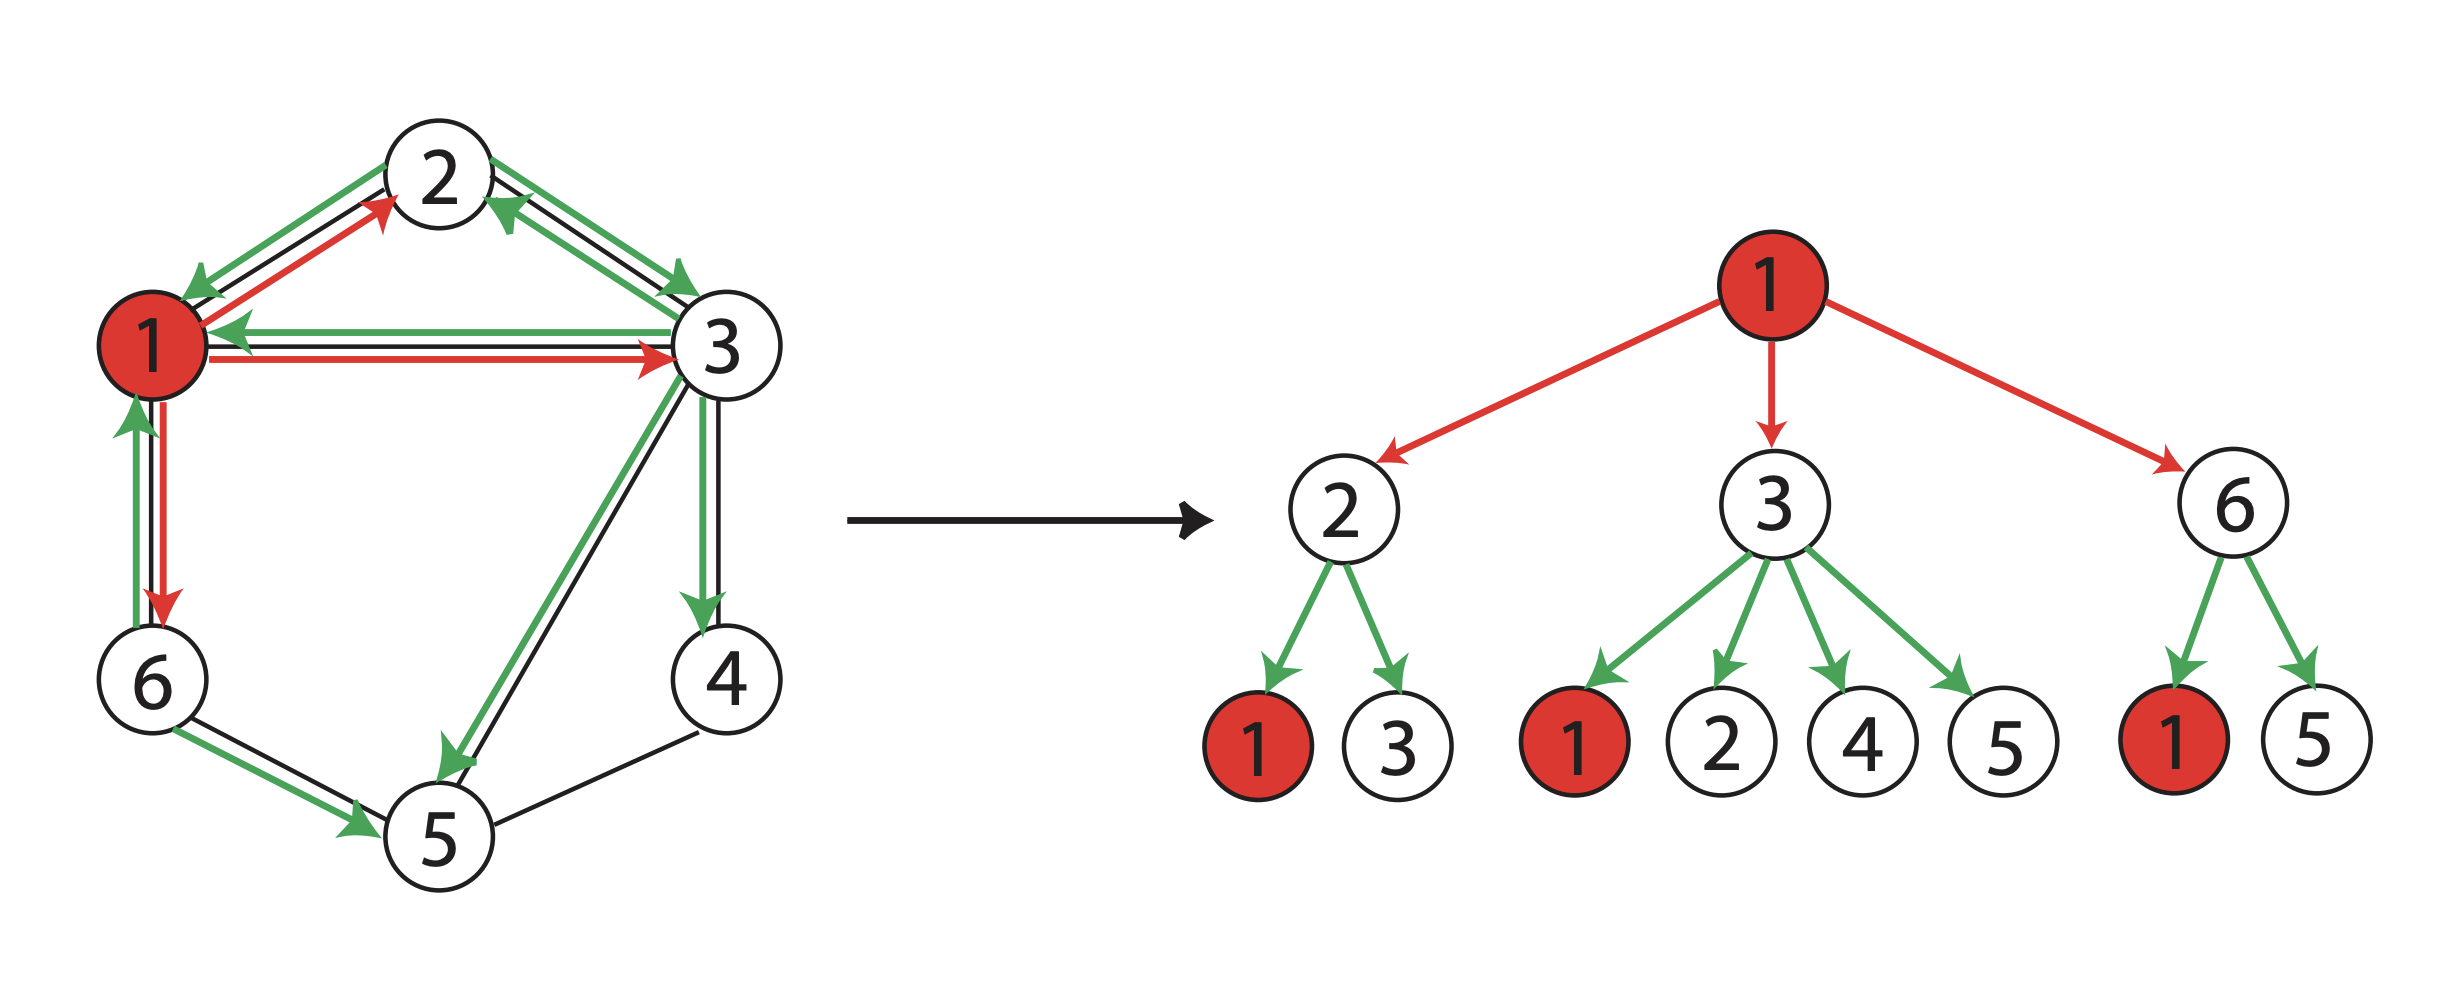
\includegraphics[width=\textwidth]{figs/tree_height_2.png}
\caption{Schematic showing the nodes reachable within two hops of the root node 1. Figure taken from \citet{SchweitzerPASCAL2011}.}
\label{fig:tree}
\end{figure}

\begin{figure}[h]
\centering
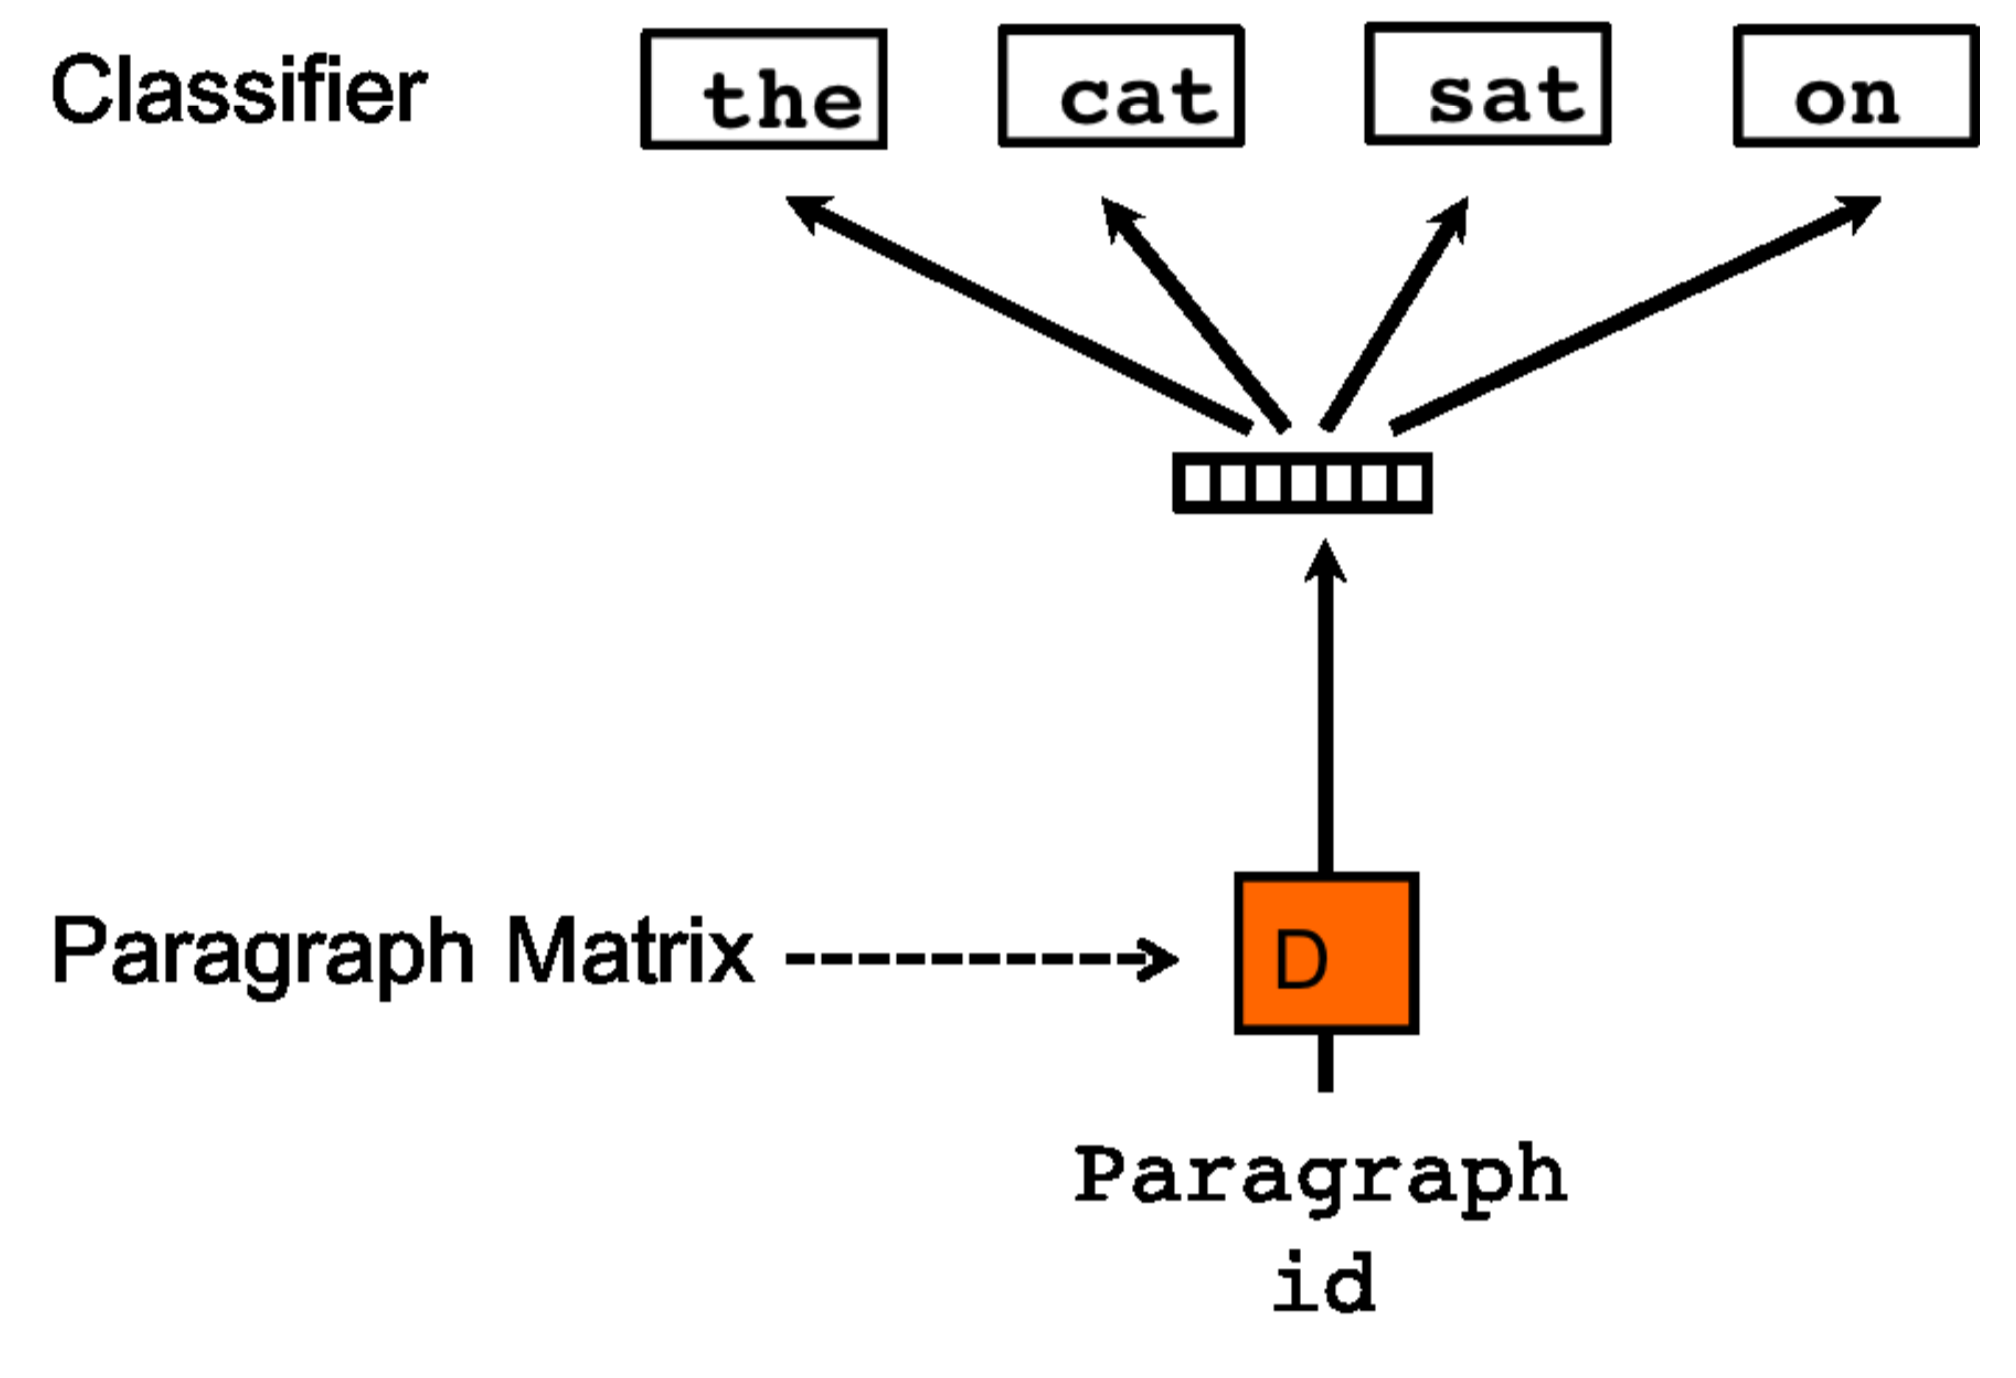
\includegraphics[width=0.6\textwidth]{figs/paragraph2vec.png}
\caption{Schematic of \textit{doc2vec} prediction taken from \citet{Le2014}. The document vector is used to predict words in a small window.}
\label{doc2vec}
\end{figure}

% histograms
\begin{figure}
\centering
\begin{subfigure}{0.45\linewidth}
    \includegraphics[width=\linewidth]{../plots/pass_plots/deg_4_dims_128_epochs_100/E_LOGP_histogram.png}
    \caption{logP}
\end{subfigure}
\begin{subfigure}{0.45\linewidth}
    \includegraphics[width=\linewidth]{../plots/pass_plots/deg_4_dims_128_epochs_100/E_WEIGHT_histogram.png}
    \caption{Weight}
\end{subfigure}
\caption{Histograms for predicted compound properties. These exhibit a heavy right skew.}
\label{fig:histograms}
\end{figure}

\begin{figure}[h]
\begin{subfigure}{0.45\textwidth}
\centering
\includegraphics[width=\textwidth]{../plots/pass_plots/deg_3_dims_256_epochs_10/is_div5.png}
\caption{10 epochs}
\label{fig:isdiv5deg_3_dims_256_epochs_10}
\end{subfigure}
\begin{subfigure}{0.45\textwidth}
\includegraphics[width=\textwidth]{../plots/pass_plots/deg_3_dims_256_epochs_100/is_div5.png}
\caption{100 epochs}
\label{fig:isdiv5deg_3_dims_256_epochs_100}
\end{subfigure}
\caption{256-dimensional embedding for degree 3 subtrees, visualized in 2 dimensions via UMAP. Diversity V Set compounds colored in orange, while other Open Set compounds colored in blue. The diversity compounds are spread well throughout the embedding space.}
\end{figure}

\begin{figure}[h]
\begin{subfigure}{0.45\textwidth}
\centering
\includegraphics[width=\textwidth]{../plots/pass_plots/deg_4_dims_128_epochs_10/is_div5.png}
\caption{10 epochs}
\label{fig:deg4_10_isdiv5}
\end{subfigure}
\begin{subfigure}{0.45\textwidth}
\includegraphics[width=\textwidth]{../plots/pass_plots/deg_4_dims_128_epochs_100/is_div5.png}
\caption{100 epochs}
\label{fig:deg4isdiv5}
\end{subfigure}
\caption{128-dimensional embedding for degree 4 subtrees, visualized in 2 dimensions via UMAP. Diversity V Set compounds colored in orange, while other Open Set compounds colored in blue. The diversity compounds are spread well throughout the embedding space.}
\end{figure}

%%%%%%%%%%%%%%%%%%%%%%%%

\begin{figure*}
\centering

\begin{subfigure}{0.45\textwidth}
    \includegraphics[width=\linewidth]{../plots/pass_plots/deg_3_dims_256_epochs_10/E_LOGP.png}
    \caption{logP}
\end{subfigure}
\begin{subfigure}{0.45\textwidth}
    \includegraphics[width=\linewidth]{../plots/pass_plots/deg_3_dims_256_epochs_10/E_WEIGHT.png}
    \caption{Weight}
\end{subfigure}
\begin{subfigure}{0.45\textwidth}
    \includegraphics[width=\linewidth]{../plots/pass_plots/deg_3_dims_256_epochs_10/Predicted_Activity_Antiinflammatory.png}
    \caption{Antiinflammatory}
\end{subfigure}
\begin{subfigure}{0.45\textwidth}
    \includegraphics[width=\linewidth]{../plots/pass_plots/deg_3_dims_256_epochs_10/Predicted_Activity_Carcinogenic.png}
    \caption{Carcinogenic}
\end{subfigure}
\begin{subfigure}{0.45\textwidth}
    \includegraphics[width=\linewidth]{../plots/pass_plots/deg_3_dims_256_epochs_10/Predicted_Activity_Immunostimulant.png}
    \caption{Immunostimulant}
\end{subfigure}
\begin{subfigure}{0.45\textwidth}
    \includegraphics[width=\linewidth]{../plots/pass_plots/deg_3_dims_256_epochs_10/Predicted_Activity_Immunosuppressant.png}
    \caption{Immunosuppressant}
\end{subfigure}
\caption{256-dimensional embedding for degree 3 subtrees trained for 10 epochs}
\label{fig:deg_3_dims_256_epochs_10}
\end{figure*}

%%%%%%%%%%%%%%%%%%%%%%%%%%%%

\begin{figure*}
\centering

\begin{subfigure}{0.45\textwidth}
    \includegraphics[width=\linewidth]{../plots/pass_plots/deg_3_dims_256_epochs_100/E_LOGP.png}
    \caption{logP}
\end{subfigure}
\begin{subfigure}{0.45\textwidth}
    \includegraphics[width=\linewidth]{../plots/pass_plots/deg_3_dims_256_epochs_100/E_WEIGHT.png}
    \caption{Weight}
\end{subfigure}
\begin{subfigure}{0.45\textwidth}
    \includegraphics[width=\linewidth]{../plots/pass_plots/deg_3_dims_256_epochs_100/Predicted_Activity_Antiinflammatory.png}
    \caption{Antiinflammatory}
\end{subfigure}
\begin{subfigure}{0.45\textwidth}
    \includegraphics[width=\linewidth]{../plots/pass_plots/deg_3_dims_256_epochs_100/Predicted_Activity_Carcinogenic.png}
    \caption{Carcinogenic}
\end{subfigure}
\begin{subfigure}{0.45\textwidth}
    \includegraphics[width=\linewidth]{../plots/pass_plots/deg_3_dims_256_epochs_100/Predicted_Activity_Immunostimulant.png}
    \caption{Immunostimulant}
\end{subfigure}
\begin{subfigure}{0.45\textwidth}
    \includegraphics[width=\linewidth]{../plots/pass_plots/deg_3_dims_256_epochs_100/Predicted_Activity_Immunosuppressant.png}
    \caption{Immunosuppressant}
\end{subfigure}
\caption{256-dimensional embedding for degree 3 subtrees trained for 100 epochs.}
\label{fig:deg_3_dims_256_epochs_100}
\end{figure*}

%%%%%%%%%%%%%%%%%%%%

\begin{figure*}
\centering

\begin{subfigure}{0.45\textwidth}
    \includegraphics[width=\linewidth]{../plots/pass_plots/deg_4_dims_128_epochs_10/E_LOGP.png}
    \caption{logP}
\end{subfigure}
\begin{subfigure}{0.45\textwidth}
    \includegraphics[width=\linewidth]{../plots/pass_plots/deg_4_dims_128_epochs_10/E_WEIGHT.png}
    \caption{Weight}
\end{subfigure}
\begin{subfigure}{0.45\textwidth}
    \includegraphics[width=\linewidth]{../plots/pass_plots/deg_4_dims_128_epochs_10/Predicted_Activity_Antiinflammatory.png}
    \caption{Antiinflammatory}
\end{subfigure}
\begin{subfigure}{0.45\textwidth}
    \includegraphics[width=\linewidth]{../plots/pass_plots/deg_4_dims_128_epochs_10/Predicted_Activity_Carcinogenic.png}
    \caption{Carcinogenic}
\end{subfigure}
\begin{subfigure}{0.45\textwidth}
    \includegraphics[width=\linewidth]{../plots/pass_plots/deg_4_dims_128_epochs_10/Predicted_Activity_Immunostimulant.png}
    \caption{Immunostimulant}
\end{subfigure}
\begin{subfigure}{0.45\textwidth}
    \includegraphics[width=\linewidth]{../plots/pass_plots/deg_4_dims_128_epochs_10/Predicted_Activity_Immunosuppressant.png}
    \caption{Immunosuppressant}
\end{subfigure}
\caption{128-dimensional embedding for degree 4 subtrees trained for 10 epochs.}
\label{fig:deg_4_dims_128_epochs_10}
\end{figure*}

%%%%%%%%%%%%%%%%%%%%%%%%%%%%%%%%%%%%

\begin{figure*}
\centering

\begin{subfigure}{0.45\textwidth}
    \includegraphics[width=\linewidth]{../plots/pass_plots/deg_4_dims_128_epochs_100/E_LOGP.png}
    \caption{logP}
\end{subfigure}
\begin{subfigure}{0.45\textwidth}
    \includegraphics[width=\linewidth]{../plots/pass_plots/deg_4_dims_128_epochs_100/E_WEIGHT.png}
    \caption{Weight}
\end{subfigure}
\begin{subfigure}{0.45\textwidth}
    \includegraphics[width=\linewidth]{../plots/pass_plots/deg_4_dims_128_epochs_100/Predicted_Activity_Antiinflammatory.png}
    \caption{Antiinflammatory}
\end{subfigure}
\begin{subfigure}{0.45\textwidth}
    \includegraphics[width=\linewidth]{../plots/pass_plots/deg_4_dims_128_epochs_100/Predicted_Activity_Carcinogenic.png}
    \caption{Carcinogenic}
\end{subfigure}
\begin{subfigure}{0.45\textwidth}
    \includegraphics[width=\linewidth]{../plots/pass_plots/deg_4_dims_128_epochs_100/Predicted_Activity_Immunostimulant.png}
    \caption{Immunostimulant}
\end{subfigure}
\begin{subfigure}{0.45\textwidth}
    \includegraphics[width=\linewidth]{../plots/pass_plots/deg_4_dims_128_epochs_100/Predicted_Activity_Immunosuppressant.png}
    \caption{Immunosuppressant}
\end{subfigure}
\caption{128-dimensional embedding for degree 4 subtrees trained for 100 epochs.}
\label{fig:deg_4_dims_128_epochs_100}
\end{figure*}



\end{document}
